\documentclass[areasetadvanced]{scrartcl}

\usepackage[utf8]{inputenc}
\usepackage[T2A]{fontenc}
\usepackage[english,russian]{babel}
\usepackage{xcolor}

\usepackage[footskip=1cm,left=25mm, right=15mm, top=20mm, bottom=20mm]{geometry}
\usepackage{setspace}
\usepackage{amsmath, amssymb} 
\usepackage{graphicx}
\usepackage{tikz}
\usetikzlibrary{arrows.meta}
\usepackage{float}
\usepackage{dashrule}
\usepackage{fancyhdr} 
\usepackage{hyperref} 
\usepackage{parskip}
\usepackage{textcomp, enumitem}
\usepackage{indentfirst}
\usepackage{graphicx}
\usepackage{algorithm}
\usepackage{algpseudocode}
\usepackage{array} 
\usepackage{geometry}
\usepackage{afterpage}
\usepackage{minted}
\setcounter{secnumdepth}{3} 
\setcounter{tocdepth}{3}    
\usepackage{listings} 
\usepackage{booktabs}
\usepackage{paracol} % параллельные колонки (левая/правая)

\newcommand{\icon}[1]{\includegraphics[height=1.2em]{#1}}

\tikzstyle{block} = [rectangle, rounded corners, minimum width=3cm, minimum height=1cm, text centered, draw=black, fill=lightgray]

\setkomafont{sectioning}{\normalfont\bfseries} 
\setkomafont{section}{\normalfont\Large\bfseries}
\setkomafont{subsection}{\normalfont\large\bfseries}
\setkomafont{subsubsection}{\normalfont\large\bfseries}
\setkomafont{paragraph}{\normalfont\large\bfseries} 
\newcommand{\twosideheading}[2]{%
  \noindent
  \begin{minipage}[t]{0.5\textwidth}\raggedright\small #1\end{minipage}%
  \begin{minipage}[t]{0.5\textwidth}\raggedleft\Large\bfseries #2\end{minipage}\\[-0.2em]
  \hrule
  \vspace{0.8em}
}
\lstset{
  language=Haskell,
  basicstyle=\ttfamily\small,
  keywordstyle=\color{blue}\bfseries,
  stringstyle=\color{red},
  commentstyle=\color{green!70!black},
  numbers=left,
  numberstyle=\tiny,
  stepnumber=1,
  numbersep=10pt,
  showstringspaces=false,
  breaklines=true,
  frame=single
}

\lstdefinelanguage{Lua}{
    keywords={function, end, if, then, else, elseif, for, while, do, repeat, until, break, return, local, and, or, not, true, false, nil},
    keywordstyle=\color{blue}\bfseries,
    stringstyle=\color{red},
    commentstyle=\color{green!70!black},
    morestring=[s]{"}{"},
    morestring=[s]{'}{'},
    morecomment=[l]{--},
    morecomment=[s]{--[[}{]]},
    basicstyle=\ttfamily\small,
    numbers=left,
    numberstyle=\tiny,
    stepnumber=1,
    numbersep=10pt,
    showstringspaces=false,
    breaklines=true,
    frame=single
}

\lstdefinestyle{py}{
    language=Python,
    basicstyle=\ttfamily\small,
    keywordstyle=\color{blue}\bfseries,
    stringstyle=\color{red},
    commentstyle=\color{green!70!black},
    numbers=left,
    numberstyle=\tiny,
    stepnumber=1,
    numbersep=10pt,
    showstringspaces=false,
    breaklines=true,
    frame=single
}

\setlength{\parindent}{1.25cm}
\setcounter{tocdepth}{3}
\begin{document}
\sloppy
	\thispagestyle{empty}
	\begin{center}
		\large{МИНОБРНАУКИ РОССИИ} \par
		\vspace{0.3cm}
		\normalsize
		{ФЕДЕРАЛЬНОЕ ГОСУДАРСТВЕННОЕ АВТОНОМНОЕ ОБРАЗОВАТЕЛЬНОЕ УЧРЕЖДЕНИЕ ВЫСШЕГО ОБРАЗОВАНИЯ} \par
		\vspace{0.3cm}
		\textbf{\guillemotleft САНКТ-ПЕТЕРБУРГСКИЙ ПОЛИТЕХНИЧЕСКИЙ}
		\textbf{УНИВЕРСИТЕТ ПЕТРА ВЕЛИКОГО\guillemotright} \par
		\vspace{0.3cm}
		{Институт компьютерных наук и кибербезопасности}\par
		{Высшая школа технологий искусственного интеллекта}\par
	\end{center}
	\vfill
	\begin{center}
		{\large Отчёт по дисциплине \guillemotleft Генетические алгоритмы\guillemotright}\par
		\vspace{1cm}
		\Huge \guillemotleft Лабораторная работа №1\guillemotright\par
		\vspace{0.5cm}
		{\huge Простой генетический алгоритм \\
        Вариант №17}\par
	\end{center}
	\vfill
	\begin{flushleft}
		Студент: \hspace{1.8cm} \rule[0pt]{2.5cm}{0.5pt}\hfill Салимли Айзек Мухтар Оглы\par
		\vspace{1.5cm}
		Преподаватель: \hspace{0.55cm} \rule[0pt]{2.5cm}{0.5pt}\hfill  Большаков Александр Афанасьевич
	\end{flushleft}
	\vspace{0.5cm}
	\begin{flushright}
		\guillemotleft \rule[0pt]{0.8cm}{0.5pt}\guillemotright \rule[0pt]{2cm}{0.5pt} 20\rule[0pt]{0.5cm}{0.5pt} г.
	\end{flushright}
	\vfill
	\begin{center}
		Санкт-Петербург, 2025
	\end{center}
	\newpage
	\tableofcontents
	\newpage

\section*{Введение}
\addcontentsline{toc}{section}{Введение}

Генетические алгоритмы (ГА) используют принципы и терминологию, заимствованные у биологической науки генетики. В ГА каждая особь представляет потенциальное решение некоторой проблемы. В классическом ГА особь кодируется строкой двоичных символов хромосомой, каждый бит которой называется геном. Множество особей потенциальных решений составляет популяцию. Поиск (суб)оптимального решения проблемы выполняется в процессе эволюции популяции - последовательного преобразования одного конечного множества решений в другое с помощью генетических операторов репродукции, кроссовера и мутации.

Предварительно простой ГА случайным образом генерирует начальную популяцию строк (хромосом). Затем алгоритм генерирует следующее поколение (популяцию), с помощью трех основных генетических операторов:

\begin{enumerate}
	\item Оператор репродукции (ОР);
	\item Оператор скрещивания (кроссовера, ОК);
	\item Оператор мутации (ОМ).
\end{enumerate}

ГА работает до тех пор, пока не будет выполнено заданное количество поколений (итераций) процесса эволюции или на некоторой генерации будет получено заданное качество или вследствие преждевременной сходимости при попадании в некоторый локальный оптимум. На Рис. 1 представлен простой генетический алгоритм.

\begin{figure}[H]
	\centering
	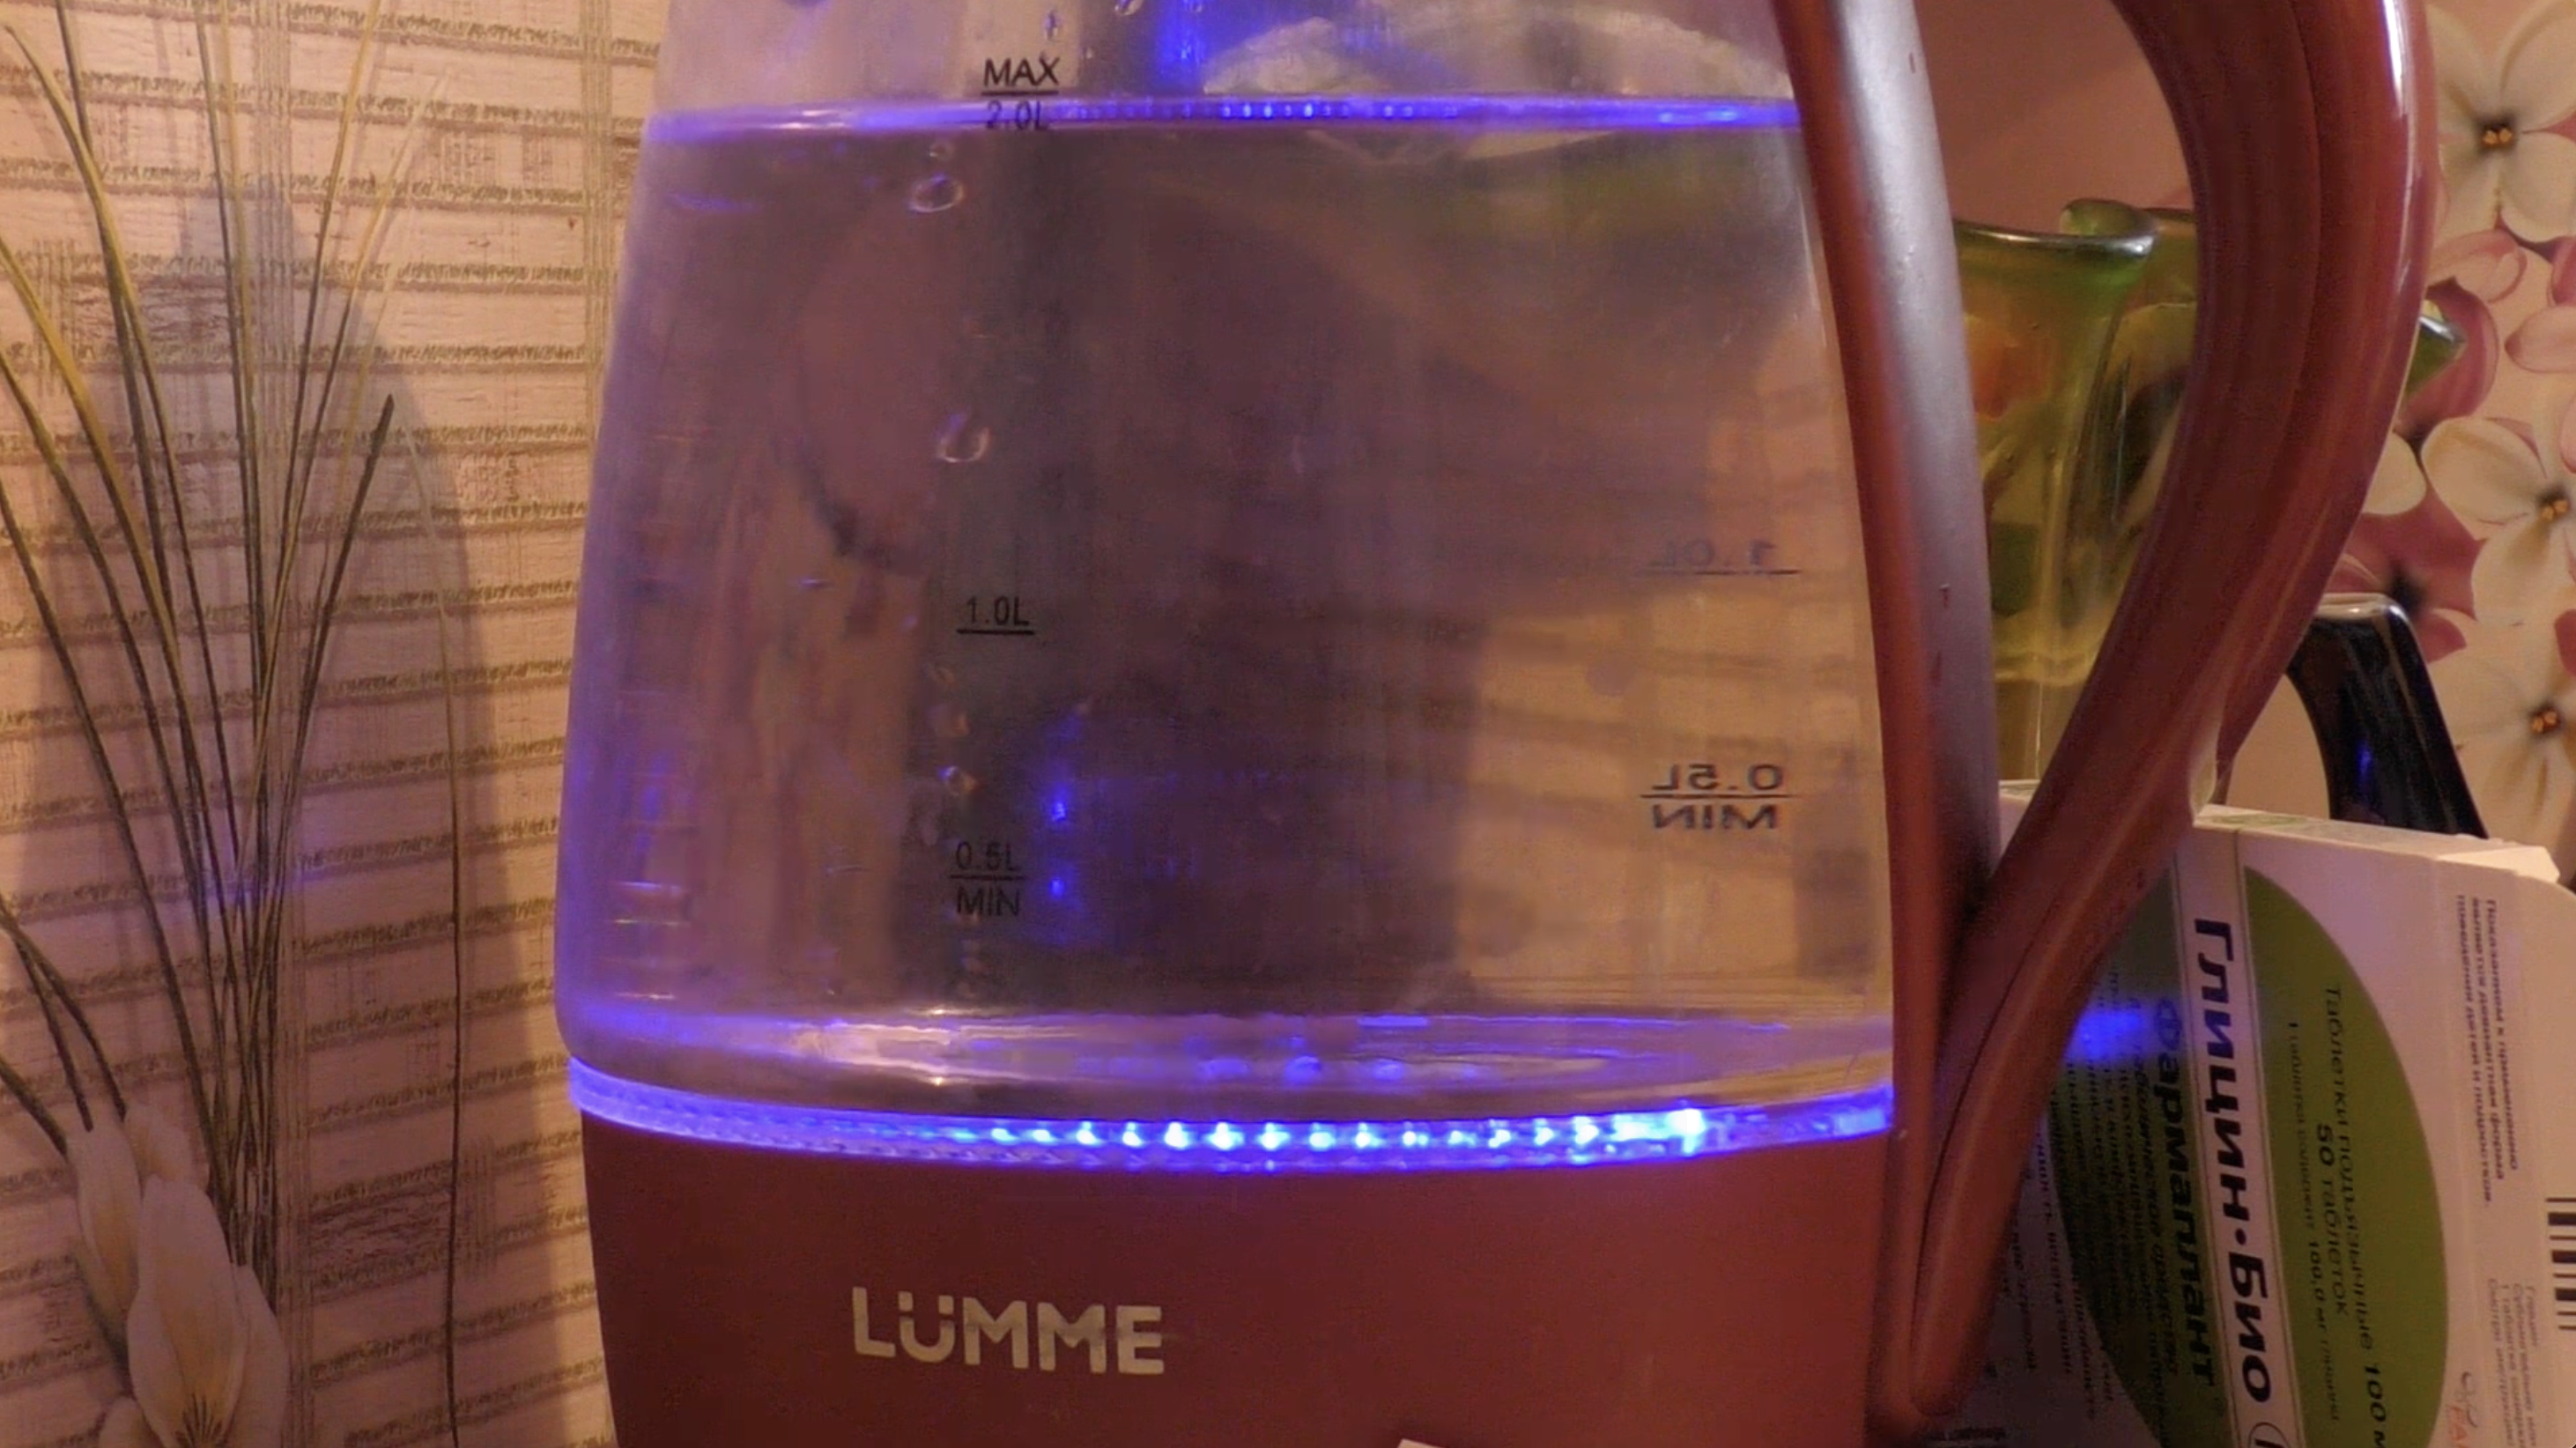
\includegraphics[width=0.4\textwidth]{img/image.png}
	\caption{Простой генетический алгоритм}
	\label{fig:GA}
\end{figure}

\newpage
\section{Постановка задачи}

\begin{itemize}
	\item Изучить теоритический материал;
	\item Выбрать индивидуальный вариант задания;
	\item Рассмотреть способы выполнения операторов репродукции, скрещивания и мутации;
	\item Реализовать программу, на выбранном языке программирования с комментариями и выводами.
\end{itemize}
\vspace{0.5cm}
\textbf{Индивидуальное задание: №17} \\
\vspace{0.5cm}
\textbf{Дано:} Функция одной переменной $f(x) = \frac{\cos(\exp{(x)})}{\sin({\ln{(x)}})}$, промежуток нахождения решения: $x \in [2,4]$.
\vspace{0.5cm}
\textbf{Требуется:} 
\begin{enumerate}
	\item Разобрать простой генетический алгоритм для нахождения минимума функции на промежутке $[2,4]$;
	\item Исследовать зависимость времени поиска, числа поколений и точности нахождения решения от числа особей в популяции и вероятность кроссинговера и мутации;
	\item Визуализировать результаты, графиками функции с указанием найденного экстремума для каждого поколения;
	\item Сравнить полученные результаты с действительными значениями.
\end{enumerate}
\vspace{0.5cm}
\textbf{Ограничения:} 
\begin{enumerate}
	\item $min \texttt{ } f(x) = \frac{\cos(\exp{(x)})}{\sin({\ln{(x)}})} \approx -1.3847$;
	\item точность: три знака после запятой;
\end{enumerate}

\newpage
\section{Определения}
\textbf{Ген} - элементарный код в хромосоме $s_i$, называемый также признаком или детектором (в классическом ГА $s_i$ = 0, 1). 

\textbf{Хромосома} - упорядоченная последовательность генов в виде закодированной структуры данных $S = (s_1, s_2, \ldots, s_n)$, определяющая решение (в простейшем случае двоичная последовательность строка, где $s_i$ = 0, 1).

\textbf{Локус} - местоположение (позиция, номер бита) данного гена в хромосоме.

\textbf{Аллель} - значение, которое принимает данный ген (например, 0 или 1).

\textbf{Особь} - одно потенциальное решение задачи (представляемое хромосомой).

\textbf{Популяция} - множество особей (хромосом), представляющих потенциальные решения.

\textbf{Поколение} - текущая популяция ГА на данной итерации алгоритма.

\textbf{Генотип} - набор хромосом данной особи. В популяции могут использоваться как отдельные хромосомы, так и целые генотипы.

\textbf{Генофонд} - множество всех возможных генотипов.

\textbf{Фенотип} - набор значений, соответствующий данному генотипу. Это декодированное множество параметров задачи (например, десятичное значение x, соответствующее двоичному коду).

\textbf{Размер популяции} - число особей в популяции.

\textbf{Число поколений} - количество итераций, в течение которых производится поиск.

\textbf{Селекция} - совокупность правил, определяющих выживание особей на основе значений целевой функции.

\textbf{Эволюция популяции} - чередование поколений, в которых хромосомы изменяют свои признаки, чтобы каждая новая популяция лучше приспосабливалась к среде.

\textbf{Фитнесс-функция} - функция полезности, определяющая меру приспособленности особи. В задачах оптимизации она совпадает с целевой функцией или описывает близость к оптимальному решению.

\newpage
\section{Генетические операторы}
		\subsection{Оператор репродукции}
		Оператор репродукции - процесс копирования хромосом в промежуточную популяцию для дальнейшего размножения в соответствии со значениями фитнесс-функции. В данной работе рассматривается метод колеса рулетки. Каждой хромосоме соответствует сектор, пропорциональный значению фитнесс-функции. Хромосомы с большим значением имеют больше шансов попасть в следующее поколение.
		\subsection{Оператор скрещивания (кроссинговер)}
		Одноточечный кроссинговер выполняется следующим образом:
		\begin{enumerate}
			\item Из промежуточной популяции выбираются две хромосомы (родители).
				\begin{figure}[H]
					\centering
					\includegraphics[width=0.3\textwidth]{img/tk.png}
				\end{figure}
			\item Определяется случайная точка скрещивания $k \in [1, n-1]$, где $n$ - длина хромосомы.
				\begin{figure}[H]
					\centering
					\includegraphics[width=0.3\textwidth]{img/tk2.png}
				\end{figure}
			\item Две новые хромосомы (потомки) формируются путем обмена подстрок после точки $k$.
		\end{enumerate}
		\subsection{Оператор мутации}
		Мутация применяется с малой вероятностью $P_M \approx 0.001$:
		\begin{enumerate}
			\item В хромосоме $A = a_1a_2\ldots a_n$ выбирается случайная позиция $k$.
			\item $a_k$-й ген хромосомы инвертируется $\Rightarrow a_k^\prime = \overline{a_k}$.
		\end{enumerate}
	
\newpage
\section{Программная реализация}
В рамках лабораторной работы был реализован ноутбук \textbf{GA\_Lab\_1.ipynb}, в котором был реализован простой генетический алгоритм для нахождения минимума функции на промежутке $[2,4]$.
\begin{itemize}
	\item Редактором кода был выбран \textbf{VS Code};
	\item Для реализации генетического алгоритма был выбран язык программирования \textbf{Python 3.13.5};
	\item Для структурирования кода, был использован \textbf{Jupyter Notebook};
	\item В качестве библиотеки для визуализации была выбрана библиотека \textbf{Matplotlib}.
\end{itemize}
\textbf{Цель.} Найти минимум функции:
\[
f(x) = \frac{\cos(e^x)}{\sin(\ln x)}, \quad x \in [2, 4].
\]

\textbf{Подход.} Простой генетический алгоритм (ГА) над \textit{хромосомами} 
(каждая особь — это число $x$), с турнирной селекцией, 
арифметическим кроссовером, мутацией, элитизмом.

\textbf{Визуализация.} Печать таблицы по поколениям и графические «снимки» эволюции 
популяции поверх кривой целевой функции.

\section*{Ключевые компоненты}

\subsection*{Целевая функция $f(x)$}
\begin{verbatim}
def f(x):
    try:
        return cos(exp(x)) / sin(log(x))
    except:
        return inf
\end{verbatim}

При проблемах области определения (например, деление на почти ноль) 
возвращает $+\infty$, чтобы такие точки автоматически «проигрывали» при минимизации.

\subsection*{Конфигурация GAConfig}

\begin{itemize}
  \item Диапазон поиска: $x_{\min}=2.0$, $x_{\max}=4.0$, округление до \texttt{precision=3}.
  \item Параметры ГА: размер популяции, число поколений, вероятности кроссовера и мутации, размер турнира, элитизм.
  \item Гауссова мутация с начальными/минимальными $\sigma$.
  \item Параметр \texttt{cx\_alpha} расширяет отрезок между родителями при арифметическом кроссовере.
\end{itemize}

\subsection*{Инициализация популяции \texttt{init\_population}}

Случайные $x \in [x_{\min}, x_{\max}]$ с округлением до \texttt{precision}.  

\section*{Как работает ГА в коде}

\begin{enumerate}
  \item \textbf{Оценка приспособленности}  
  \begin{verbatim}
  fitness = evaluate(pop, f)
  \end{verbatim}
  Для минимизации используется прямое сравнение значений $f(x)$ — меньше значит лучше.
  Значение \texttt{inf} отталкивает невалидные точки.

  \item \textbf{Селекция — турнирная}  
  \begin{verbatim}
  def tournament_select(pop, fitness, k):
      # выбираем k случайных индексов, берем лучшего (min fitness)
  \end{verbatim}
  Параметр \texttt{tournament\_size} управляет «давлением отбора»: чем больше $k$, тем сильнее отбор.

  \item \textbf{Кроссовер — арифметический}  
  \begin{verbatim}
  c1, c2 = arithmetic_crossover(p1, p2, alpha=cfg.cx_alpha)
  \end{verbatim}
  Пусть $L = |p_1 - p_2|$. Потомки берутся из расширенного отрезка 
  $[p_{\min} - \alpha L,\, p_{\max} + \alpha L]$, что даёт больше разнообразия.

  \item \textbf{Мутация} 
  \begin{verbatim}
  sigma = max(sigma_floor, sigma_init * sigma_decay**gen)
  x' = x + Normal(0, sigma)
  \end{verbatim}
  В начале $\sigma$ больше (широкий поиск), затем затухает (локальное уточнение).
  Результаты ограничиваются диапазоном и округляются.

  \item \textbf{Элитизм}
  \begin{verbatim}
  elite_idx = argsort(fitness)[:elitism]
  next_pop = [pop[i] for i in elite_idx]
  \end{verbatim}
  Лучшая часть популяции без изменений переходит в следующее поколение.

  \item \textbf{Формирование нового поколения}  
  После элитизма добор: турнир → кроссовер (с вероятностью $p_c$) → мутация → добавление.  
  В конце все значения округляются и оцениваются заново.

  \item \textbf{История и останов}  
  Хранится история популяций (\texttt{pop\_history}), лучшие пары $(x, f(x))$, таблица метрик.  
  Критерий остановки — фиксированное число поколений.
\end{enumerate}

\section*{Вспомогательные части}

\begin{itemize}
  \item \textbf{Табличный лог \texttt{print\_table}} — выводит \texttt{best\_x}, \texttt{best\_f}, \texttt{mean\_f} по поколениям.
  \item \textbf{Визуализация \texttt{plot\_snapshot}} — график функции и положение популяции, текущего и предыдущего лучших.
  \item \textbf{Детерминизм.}  
  \texttt{random.seed(cfg.seed)} обеспечивает повторяемость экспериментов.
\end{itemize}
\newpage
\section{Результаты}
Ниже, на Рис. 2 - 5 представлены результаты работы генетического алгоритма.

\begin{itemize}
	\item \(N = 20\) — размер популяции;
	\item \(p_c = 0.85\) — вероятность кроссинговера;
	\item \(p_m = 0.12\) — вероятность мутации;
	\item поиск на отрезке \([2,4]\) с округлением до \(10^{-3}\);
  \end{itemize}
  
  С каждым поколением точность найденного минимума возрастает:  
  — средняя приспособленность популяции снижается,  
  — лучшая особь стабильно улучшается.
  
  На ранних поколениях (например, \(g=0,5\)) особи покрывают значительную часть области поиска; к эволюции (\(g\approx10\)) популяция «конденсируется» в окрестности экстремума; к финалу (\(g=15\)) достигается заданная точность (округление \(10^{-3}\)), а лучшая особь находится вблизи минимума.
  
  Визуализация включает по-поколенческие снимки: график функции, текущую популяцию, лучшую особь текущего поколения (звёздочка) и лучшую особь предыдущего поколения (для сравнения).  
  Алгоритм завершает работу по фиксированному числу поколений (\(15\));  
  помимо графиков печатается таблица с метриками по поколениям: \texttt{best\_x}, \texttt{best\_f}, \texttt{mean\_f}.

\begin{figure}[H]
	\centering
	\includegraphics[width=0.7\textwidth]{img/image copy.png}
	\caption{Поколение 0 - начальная популяция}
	\label{fig:results1}
\end{figure}

\begin{figure}[H]
	\centering
	\includegraphics[width=0.7\textwidth]{img/image copy 2.png}
	\caption{Поколение 5}
	\label{fig:results2}
\end{figure}

\begin{figure}[H]
	\centering
	\includegraphics[width=0.7\textwidth]{img/image copy 3.png}
	\caption{Поколение 10 - концентрация популяции}
	\label{fig:results3}
\end{figure}

\begin{figure}[H]
	\centering
	\includegraphics[width=0.7\textwidth]{img/image copy 5.png}
	\caption{Финальное поколение 15}
	\label{fig:results5}
\end{figure}

\newpage
\section{Выводы и исследование}
\section*{Анализ результатов работы}
В эксперименте использовались следующие параметры генетического алгоритма:
\[
N=20,\qquad p_c=0.85,\qquad p_m=0.12.
\]
Алгоритм находит минимум функции  
\[
f(x) = \frac{\cos(e^x)}{\sin(\ln x)},\quad x\in[2,4]
\]  
достаточно быстро, и результаты близки к тем, что получаются при плотном сканировании (reference: \(x\approx 2.2385,\; f\approx -1.38478\)).

\paragraph{Динамика сходимости.}
Уже к поколению \(g=10\) лучшая особь демонстрирует значение минимума; к \(g=15\) популяция практически полностью концентрируется в его окрестности. Динамика значений лучшего и среднего по популяции представлена в таблице~\ref{tab:ga_runs}.

\begin{table}[H]
  \centering
  \caption{Эволюция лучшей и средней приспособленности по поколениям}
  \label{tab:ga_runs}
  \begin{tabular}{r r r r r}
    \toprule
    Gen & Best\_x & Best\_f & Mean\_f & Time(s) \\
    \midrule
     0 & 2.302 & ‐1.137430 & ‐0.308400 & 0.0006 \\
     1 & 2.757 & ‐1.176649 & ‐0.856102 & 0.0001 \\
     2 & 2.756 & ‐1.177595 & ‐0.263769 & 0.0001 \\
     3 & 2.268 & ‐1.331403 & ‐1.160674 & 0.0001 \\
     4 & 2.246 & ‐1.381351 & ‐1.144883 & 0.0001 \\
     5 & 2.244 & ‐1.382934 & ‐1.358064 & 0.0002 \\
     6 & 2.240 & \textcolor{red}{‐1.384639} & ‐1.382867 & 0.0001 \\
     7 & 2.240 & ‐1.384639 & ‐1.383304 & 0.0001 \\
     8 & 2.240 & ‐1.384639 & ‐1.384462 & 0.0003 \\
     9 & 2.240 & ‐1.384639 & ‐1.382024 & 0.0001 \\
    10 & 2.240 & ‐1.384639 & ‐1.384639 & 0.0001 \\
    11 & 2.240 & ‐1.384639 & ‐1.384639 & 0.0001 \\
    12 & 2.240 & ‐1.384639 & ‐1.382654 & 0.0001 \\
    13 & 2.240 & ‐1.384639 & ‐1.371588 & 0.0001 \\
    14 & 2.240 & ‐1.384639 & ‐1.384639 & 0.0001 \\

    \bottomrule
  \end{tabular}
\end{table}

В данном запуске использован размер популяции $N=50$.
Таблица ниже показывает динамику лучшего решения и среднего значения по популяции по поколениям.

\begin{table}[H]
\centering
\caption{Эволюция лучшего и среднего значения целевой функции ($N=50$)}
\label{tab:ga_runs_N50}
\begin{tabular}{r|r|r|r|r}
\hline
\textbf{Gen} & \textbf{Best\_x} & \textbf{Best\_f} & \textbf{Mean\_f} & \textbf{Time(s)} \\
\hline
  0 & 2.745 & -1.168921 & -0.645240 & 0.0003 \\
  1 & 2.223 & -1.370500 & -0.748739 & 0.0002 \\
  2 & 2.237 & -1.384646 & -1.189021 & 0.0002 \\
  3 & 2.238 & \textcolor{red}{-1.384764} & -1.352526 & 0.0003 \\
  4 & 2.238 & -1.384764 & -1.350280 & 0.0005 \\
  5 & 2.238 & -1.384764 & -1.361282 & 0.0002 \\
  6 & 2.238 & -1.384764 & -1.370731 & 0.0002 \\
  7 & 2.238 & -1.384764 & -1.377510 & 0.0002 \\
  8 & 2.238 & -1.384764 & -1.384757 & 0.0002 \\
  9 & 2.238 & -1.384764 & -1.381099 & 0.0002 \\
 10 & 2.238 & -1.384764 & -1.379964 & 0.0002 \\
 11 & 2.238 & -1.384764 & -1.371425 & 0.0008 \\
 12 & 2.238 & -1.384764 & -1.384676 & 0.0004 \\
 13 & 2.238 & -1.384764 & -1.381669 & 0.0003 \\
 14 & 2.238 & -1.384764 & -1.384630 & 0.0002 \\
\hline
\end{tabular}
\end{table}

Результаты популяции $N=100$

В данном запуске использован размер популяции $N=100$. Уже к поколениям $g=10\text{–}15$ лучшая особь достигает значения минимума. Однако к $g=15$ популяция ещё \emph{не полностью сконцентрировалась} в его окрестности: среднее значение по популяции остаётся заметно выше по модулю минимального.

\begin{table}[H]
\centering
\caption{Эволюция лучшего и среднего значения целевой функции ($N=100$)}
\label{tab:ga_runs_N100}
\begin{tabular}{r|r|r|r|r}
\hline
\textbf{Gen} & \textbf{Best\_x} & \textbf{Best\_f} & \textbf{Mean\_f} & \textbf{Time(s)} \\
\hline
  0 & 2.745 & -1.168921 & -0.409121 & 0.0008 \\
  1 & 2.248 & -1.379278 & -0.548675 & 0.0013 \\
  2 & 2.245 & -1.382203 & -0.759144 & 0.0004 \\
  3 & 2.240 & -1.384639 & -1.211791 & 0.0010 \\
  4 & 2.238 & \textcolor{red}{-1.384764} & -1.373112 & 0.0003 \\
  5 & 2.238 & -1.384764 & -1.361731 & 0.0004 \\
  6 & 2.238 & -1.384764 & -1.377298 & 0.0003 \\
  7 & 2.238 & -1.384764 & -1.369395 & 0.0003 \\
  8 & 2.238 & -1.384764 & -1.373058 & 0.0011 \\
  9 & 2.238 & -1.384764 & -1.379324 & 0.0008 \\
 10 & 2.238 & -1.384764 & -1.351899 & 0.0008 \\
 11 & 2.238 & -1.384764 & -1.383980 & 0.0003 \\
 12 & 2.238 & -1.384764 & -1.383903 & 0.0003 \\
 13 & 2.238 & -1.384764 & -1.381956 & 0.0003 \\
 14 & 2.238 & -1.384764 & -1.381509 & 0.0011 \\
\hline
\end{tabular}
\end{table}


\paragraph{Исследование влияния параметров.}

Для исследования влияния размера популяции и параметров генетического алгоритма были проведены эксперименты с различными конфигурациями:

\begin{itemize}
  \item \textbf{Размер популяции:} \(N \in \{20, 50, 100\}\)
  \item \textbf{Вероятность кроссовера:} \(p_c \in \{0.3, 0.5, 0.6, 0.85\}\)
  \item \textbf{Вероятность мутации:} \(p_m \in \{0.01, 0.05, 0.12, 0.2\}\)
  \item \textbf{Число поколений:} 15 (для сравнения результатов)
\end{itemize}

\subparagraph{Результаты для \(N = 20\):}
При малых популяциях повышение \(p_m\) ускоряет поиск; наилучшее время при \(p_c = 0.5\), \(p_m = 0.12\) (сходимость к поколению 8-10). Для стабильной работы оптимально \(p_c = 0.85\), \(p_m = 0.12\).

\subparagraph{Результаты для \(N = 50\):}
при умеренной мутации \(p_m \in [0.05, 0.12]\); лучшая сходимость при \(p_c = 0.85\), \(p_m = 0.05\) (сходимость к поколению 4-6). Слишком большая мутация (\(p_m = 0.2\)) резко ухудшает результаты.

\subparagraph{Результаты для \(N = 100\):}
Оптимальны низкие \(p_m\); лучший результат при \(p_c = 0.85\), \(p_m = 0.05\) (сходимость к поколению 3-5). При \(p_m = 0.2\) решение часто не находится за 15 поколений.

\subparagraph{Влияние размера популяции:}
Суммарное время часто растёт из-за большей стоимости одной итерации. При \(N = 100\) достигается быстрая сходимость (3-5 поколений), но вычислительная сложность возрастает.

\paragraph{Практические выводы:}

\begin{itemize}
  \item Для умеренных затрат времени и стабильной сходимости разумно выбирать \(N \approx 50\), \(p_c \approx 0.85\), \(p_m \approx 0.05\).
  \item Оптимальное \(p_m\) снижается с ростом \(N\): при малых популяциях полезна более агрессивная мутация, при больших — слабая.
  \item Слишком большие значения \(p_m\) и \(p_c\) могут разрушать хорошие решения и ухудшать сходимость; стоит избегать \(p_m \geq 0.2\) и высоких \(p_c\) при больших \(N\).
  \item Минимум достигается уже к поколениям \(3\div6\), после чего изменения очень малые.  
  \item Лучшее значение \(f\approx -1.38476\) близко к скановому ~\(-1.38478\), погрешность порядка \(10^{-4}\).  
  \item Среднее значение приспособленности популяции стабильно улучшается, что говорит о эффективной работе генетических операторов.
\end{itemize}


\newpage
\section{Заключение}

В ходе первой лабораторной работы:

\begin{enumerate}
	\item Был изучен теоретический материал, основная терминология ГА, генетические операторы, использующиеся в простых ГА;
	\item Реализована программа на языке Python для нахождения минимума заданной функции;
	\item Проведено исследование зависимости поколения от мощности популяции и коэффициентов кроссовера и мутации.
\end{enumerate}
\vspace{0.5cm}
В результате проведённых экспериментов было установлено, что генетический алгоритм эффективно находит минимум функции $f(x) = \frac{\cos(e^x)}{\sin(\ln x)}$ на отрезке $[2,4]$ с высокой точностью.

\vspace{0.5cm}
Оптимальные параметры для данной задачи: размер популяции $N \in \{20, 50\}$, вероятность кроссовера $p_c = 0.85$, вероятность мутации $p_m = 0.05$.

\newpage
\section{Ответ на контрольный вопрос}
\textbf{Вопрос:} Какие генетические операторы используются в ГА? \\
\textbf{Ответ:} В генетическом алгоритме используются три основных оператора:

\begin{enumerate}
	\item \textbf{Оператор репродукции (селекции)} — выбирает наиболее приспособленных особей для дальнейшего размножения. Обеспечивает сохранение лучших решений и направляет эволюцию в сторону улучшения качества популяции.
	
	\item \textbf{Оператор скрещивания (кроссовера)} — создает новых потомков путем комбинирования генетического материала двух родительских особей. Позволяет исследовать новые области пространства решений и объединять полезные признаки от разных особей.
	
	\item \textbf{Оператор мутации} — случайным образом изменяет отдельные гены в хромосомах. Предотвращает преждевременную сходимость алгоритма, обеспечивает генетическое разнообразие популяции и позволяет исследовать новые области поиска.
\end{enumerate}

\newpage
\section*{Список литературы}
\addcontentsline{toc}{section}{Список литературы}
\begin{enumerate}
	\item Методические указания по выполнению лабораторных работ к курсу "Генетические алгоритмы", 119 стр.
\end{enumerate}

\newpage
\addcontentsline{toc}{section}{Приложение А}
\twosideheading{Исходный код}{Приложение А}

% -------- Ниже — ваш код
\begin{lstlisting}[style=py,caption={Приложение А: исходный код},label={lst:appA}]
import math
import random
from dataclasses import dataclass
from typing import Callable, List, Tuple, Dict
import numpy as np
import matplotlib.pyplot as plt


def f(x: float) -> float:
    try:
        return math.cos(math.exp(x)) / math.sin(math.log(x))
    except Exception:
        return float("inf")

@dataclass
class GAConfig:
    x_min: float = 2.0
    x_max: float = 4.0
    precision: int = 3

    pop_size: int = 50
    generations: int = 60

    crossover_rate: float = 0.85
    mutation_rate: float = 0.12          
    elitism: int = 4
    tournament_size: int = 4

    sigma_init: float = 0.08
    sigma_floor: float = 0.001
    sigma_decay: float = 0.96

    cx_alpha: float = 0.10

    seed: int = 7

    avoid_min_at_start: bool = True
    avoid_window_dx: float = 0.06  

def clamp(x, a, b): return max(a, min(b, x))
def roundp(x, p): return round(x, p)

def arithmetic_crossover(p1: float, p2: float, alpha: float) -> Tuple[float, float]:
    lo, hi = (p1, p2) if p1 <= p2 else (p2, p1)
    L = hi - lo
    a = lo - alpha * L
    b = hi + alpha * L
    r = random.random()
    c1 = a + r * (b - a)
    c2 = a + (1 - r) * (b - a)
    return c1, c2

def mutate(x: float, rate: float, sigma: float, cfg: GAConfig) -> float:
    if random.random() < rate:
        x = x + random.gauss(0.0, sigma)
        x = clamp(x, cfg.x_min, cfg.x_max)
        x = roundp(x, cfg.precision)
    return x

def evaluate(pop: List[float], func: Callable[[float], float]) -> List[float]:
    return [func(x) for x in pop]

def tournament_select(pop: List[float], fitness: List[float], k: int) -> float:
    idxs = random.sample(range(len(pop)), k)
    best_idx = min(idxs, key=lambda i: fitness[i])   
    return pop[best_idx]

def dense_scan_min(x_min=2.0, x_max=4.0) -> Tuple[float, float]:
    xs = np.linspace(x_min, x_max, 40001)
    ys = np.cos(np.exp(xs)) / np.sin(np.log(xs))
    i = int(np.argmin(ys))
    return float(xs[i]), float(ys[i])

def init_population(cfg: GAConfig, forbid: Tuple[float, float] | None) -> List[float]:
    pop = []
    while len(pop) < cfg.pop_size:
        x = roundp(random.uniform(cfg.x_min, cfg.x_max), cfg.precision)
        if forbid and (forbid[0] <= x <= forbid[1]):
            continue
        pop.append(x)
    return pop

def run_ga(func: Callable[[float], float], cfg: GAConfig) -> Dict:
    random.seed(cfg.seed)

    approx_x, approx_y = dense_scan_min(cfg.x_min, cfg.x_max)
    forbid = None
    if cfg.avoid_min_at_start:
        a = clamp(approx_x - cfg.avoid_window_dx, cfg.x_min, cfg.x_max)
        b = clamp(approx_x + cfg.avoid_window_dx, cfg.x_min, cfg.x_max)
        forbid = (a, b)

    pop = init_population(cfg, forbid)
    fitness = evaluate(pop, func)

    pop_history: List[List[float]] = [pop.copy()]     
    best_history: List[Tuple[float, float]] = []      
    table_rows: List[Dict] = []

    for gen in range(cfg.generations):
        i_best = int(np.argmin(fitness))
        best_x_gen = pop[i_best]
        best_f_gen = float(fitness[i_best])

        best_history.append((best_x_gen, best_f_gen))
        table_rows.append({
            "generation": gen,
            "best_x": best_x_gen,
            "best_f": best_f_gen,
            "mean_f": float(np.mean(fitness)),
        })

        elite_idx = np.argsort(fitness)[:cfg.elitism]
        next_pop = [pop[i] for i in elite_idx]

        sigma = max(cfg.sigma_floor, cfg.sigma_init * (cfg.sigma_decay ** gen))

        while len(next_pop) < cfg.pop_size:
            p1 = tournament_select(pop, fitness, cfg.tournament_size)
            p2 = tournament_select(pop, fitness, cfg.tournament_size)

            if random.random() < cfg.crossover_rate:
                c1, c2 = arithmetic_crossover(p1, p2, cfg.cx_alpha)
            else:
                c1, c2 = p1, p2

            c1 = mutate(c1, cfg.mutation_rate, sigma, cfg)
            c2 = mutate(c2, cfg.mutation_rate, sigma, cfg)

            next_pop.extend([c1, c2])

        pop = [roundp(clamp(x, cfg.x_min, cfg.x_max), cfg.precision) for x in next_pop[:cfg.pop_size]]
        fitness = evaluate(pop, func)
        pop_history.append(pop.copy())

    final_best = best_history[-1]
    return {
        "pop_history": pop_history,
        "best_history": best_history,
        "final_best": final_best,
        "table": table_rows,
        "approx_min": (approx_x, approx_y),
        "cfg": cfg,
    }

def compute_curve(x_min: float, x_max: float):
    xs = np.linspace(x_min, x_max, 2000)
    ys = np.cos(np.exp(xs)) / np.sin(np.log(xs))
    return xs, ys

def plot_snapshot(xs, ys, gen_idx: int, pop_history: List[List[float]], best_history: List[Tuple[float, float]]):
    pop_cur = pop_history[gen_idx]
    best_cur_x, best_cur_f = best_history[gen_idx] if gen_idx < len(best_history) else best_history[-1]
    prev_best = best_history[gen_idx - 1] if gen_idx - 1 >= 0 else None

    plt.figure(figsize=(9, 5))
    plt.plot(xs, ys, label="Target function")
    plt.scatter(pop_cur, [f(x) for x in pop_cur], s=28, label=f"Population gen {gen_idx}", color="blue")
    plt.scatter([best_cur_x], [best_cur_f], s=140, marker="*", color="red", label="Best (cur)")
    if prev_best is not None:
        plt.scatter([prev_best[0]], [prev_best[1]], s=60, color="gray", label="Best (prev)")
    plt.title(f"Generation {gen_idx} best f={best_cur_f:.6f}")
    plt.xlabel("x"); plt.ylabel("f(x)")
    plt.grid(True); plt.legend()
    plt.tight_layout()
    plt.show()

def print_table(rows: List[Dict]) -> None:
    header = f"{'Gen':>4} | {'Best_x':>8} | {'Best_f':>12} | {'Mean_f':>12}"
    print("\n" + header)
    print("-" * len(header))
    for r in rows:
        print(f"{r['generation']:>4} | {r['best_x']:>8.3f} | {r['best_f']:>12.6f} | {r['mean_f']:>12.6f}")

def main():
    cfg = GAConfig(
        pop_size=100,
        generations=15,
        crossover_rate=0.85,
        mutation_rate=0.05,
        elitism=4,
        tournament_size=4,
        precision=3,
        sigma_init=0.08,
        sigma_floor=0.001,
        sigma_decay=0.96,
        cx_alpha=0.10,
        seed=7,
        avoid_min_at_start=True,
        avoid_window_dx=0.06,
    )

    res = run_ga(f, cfg)
    pop_history = res["pop_history"]
    best_history = res["best_history"]
    rows = res["table"]
    approx_x, approx_y = res["approx_min"]

    print_table(rows)

    xs, ys = compute_curve(cfg.x_min, cfg.x_max)

    gens_to_show = [0, 5, 10, 20, 30, 40, 50, 60]
    gens_to_show = [g for g in gens_to_show if 0 <= g < len(pop_history)]
    if (len(pop_history)-1) not in gens_to_show:
        gens_to_show.append(len(pop_history)-1)

    for g in gens_to_show:
        plot_snapshot(xs, ys, g, pop_history, best_history)


if __name__ == "__main__":
    main()
\end{lstlisting}
\end{document}